\chapter{Design}\label{ch:design}

To achieve high performance I/O on seL4, this thesis will extend the current seL4 Device Driver Framework prototype 
to securely support multiple client applications on a multi-core system. While doing so, 
we will evaluate the sDDF design while improving any bottlenecks in the current implementation
and optimise the system for high performance networking systems.

When extending the sDDF, we wish to maintain the current prototype's design goals. 
Specifically, these are:
\begin{itemize}
\item \textbf{Radical Simplicity}: Each component in the framework should be kept as simple as possible. While verification is outside the scope
of this thesis, keeping each component simple will aid any future verification effort while assisting developers to reason about it.
\item \textbf{Strict separation of concerns}: Each component has one and only one job to do. 
\item \textbf{Swappable policy}: Any policy enforced by the framework should be swappable for another policy for different use cases.
This enables the framework to be flexible and support different use cases while keeping the implementation simple.
\item \textbf{Secure}: The framework should be secure by taking advantage of the security properties provided by seL4. seL4 guarantees
complete isolation of user-level components, and its capability system provides fine grained access control. Untrusted clients must not be able
to interfere with one another, nor any of the trusted shared components such as the multiplexers. 
\item \textbf{Performance}: The solution should be performance competitive with the current prototype,
as well as with other existing I/O frameworks (see \autoref{ch:related_work}).
\end{itemize}

To accomplish our goal, we need to:
\begin{enumerate}
    \item Implement policies for the multiplexers, \autoref{s:mux_pol}
    \item Support broadcast protocols, \autoref{s:arp}
    \item Support different client applications that imitate different use cases, \autoref{s:client_apps}
    \item Support execution across multiple CPUs, \autoref{s:multicore}
    \item Perform a threat analysis of the framework to outline, and where possible, improve any
         security vulnerabilities in our design, \autoref{s:security}
    \item Evaluate and optimise: evaluate the solution by benchmarking the system throughout development 
    and improve any performance bottlenecks.
\end{enumerate}

\section{Multiplexer Policy} \label{s:mux_pol}

A multiplexer servicing multiple components inherently requires a policy to
determine the order in which it will process work. Rather than designing a generic policy
that aims to cater to all possible use-cases, we instead
design several different multiplexers that implement a simple policy for a specific use-case. 

Both the Rx and Tx multiplexers are trusted components,
and thus are kept intentionally simple to leave them accessible to formal verification.
The main tasks of the multiplexers, regardless of policy implemented, are as follows:

\begin{itemize}
    \item Given a virtual address from the client/copier, translate it to a physical address before
            handing it over to the driver.
    \item Given a physical address from the driver, translate it to a virtual address before
            handing it over to the client/copier.
    \item Sanitise any buffer addresses from the client before forwarding them.
    \item Sanitise any addresses from the driver. 
    \item Transmit buffers belong to the client, and therefore all free buffers on the transmit path
            must be returned to the appropriate client.
    \item Receive buffers belong to the driver, and therefore all free buffers on the receive path
            must be returned to the driver.
\end{itemize}

%    \item The transmit multiplexer has the ability to sanitise the Ethernet header of outgoing packets
%to ensure the destination MAC address is well formed and will not cause issues
%on the network. Modern NICs are capable of sanitising headers of outgoing packets,
%%but many systems may require a design whereby the NIC is not trusted to perform this check 
%and thus it should be done in software.

\subsection{Receive Policy}\label{s:rx_policy}

All incoming packets are processed in FIFO order. The multiplexer contains a 
mapping of virtualised client MAC addresses and client queues. After dequeuing an incoming packet,
the multiplexer must first invalidate the cache (to ensure subsequent reads are fetched again from memory)
and read the packet header. The packet header contains the destination MAC address and if the packet is
addressed to a client on the system, the buffer address is forwarded to the appropriate client. 
If a client's Receive Used (RxU) queue is full, the multiplexer drops the packet and the buffer address is returned to
the driver. This can be prevented for higher priority clients by appropriate choice of client's RxU queue
sizes. Appropriate sizes can be selected based on experiments discussed in \autoref{ch:evaluation}.

The multiplexer must also return free buffers to the driver to be reused again. If a clients Receive Free
(RxF) queue is full, the multiplexer could stall the client while it waits to enqueue free buffers. Should this be the case,
the order in which the multiplexer processes the client RxF queue contains policy as it may
unblock clients. We propose instead to ensure the clients RxF queue is the same size as the number
of receive buffers circulating and thus prevent the client becoming blocked on waiting for this queue to be
processed. This design removes the need for policy on processing free buffers. \\ 

\subsection{Transmit Policy}

All incoming requests from clients are processed subject to a particular policy. 
We implement 3 different policies in \autoref{ch:implementation}:
\begin{enumerate}
    \item \textbf{Round-robin}: whereby the multiplexer processes an outgoing request one at a time, alternating between clients.
    \item \textbf{Priority-based}: whereby the multiplexer prioritises client requests as per their given priority, processing as many
    requests as available for the highest priority client possible. 
    \item \textbf{Throughput-based}: whereby the multiplexer limits the available outgoing bandwidth per client at a time.
\end{enumerate}

The transmit multiplexer also returns
free buffers from the driver to the client in FIFO order, regardless of policy implemented on
processing transmit requests. However, the multiplexer has no way of knowing which client
a particular buffer belongs to before it has been dequeued. Should a particular client's 
Transmit Free (TxF) queue be full, the multiplexer could become blocked waiting to enqueue
a free buffer. We propose client TxF queues are at least 
the size of the number of buffers belonging to that client in order to prevent this. \\ 
Similarly, the drivers Transmit Used (TxU) queue should be at least the size of the sum of 
all client transmit buffers. This ensures the multiplexer will not become blocked on this queue
and thus disrupt the policy implemented to process client requests. \\ 

\subsection{Enforcing Policy Through System Design}
Depending on the greater system design, we expect some transmit policies not to work.
For example, given a single-core configuration, the higher priority multiplexer will
always be invoked as soon as a client has made a request to transmit. This means that
we can assume any other clients do not yet wish to transmit, or have not yet had the
opportunity to run to make a request. Therefore, the multiplexer does not need to 
consider all the client queues when invoked and can just service requests made
by the client that signalled. To enforce policy on multiple clients in such a scenario,
we rely on appropriate choices of client queue sizes and the scheduling parameters
of each client. For example, to enforce a round-robin policy on two clients, we run both clients
at equal priorities, and limit their TxU queues to one. This ensures
that each client will be stalled until its single request has been processed, and
another client will have the opportunity to run in the interim. The multiplexer will
then only process a single request per client at a time, though at the detriment of performance.\\
Similarly, should we require a priority based policy, we can assign appropriate priorities
to the clients scheduling parameters and limit lower priority client's queue sizes, thus relying on the scheduling
of the system to enforce this policy.\\
Finally, we can limit the client's queue sizes on both the transmit and/or receive paths
to limit the amount of either transmit and/or receive throughput available to each client.
Appropriate sizes can be selected based on experiments discussed in \autoref{ch:evaluation}.\\ 

\subsection{Design Constraints}

Our multiplexer design has introduced 2 small constraints that will impose on system design. To summarise,
these are:

\begin{itemize}
    \item All client's RxF queues must be the same size or greater than the total number of receive buffers circulating in the system. 
        This is to prevent a client from becoming blocked, waiting for this queue to be processed and thus requiring further policy 
        in the Rx multiplexer to handle free buffers. This constraint has no impact on the implementation, but must be considered 
        when configuring queue sizes across the system. 
    \item All client's TxF queues must be the same size or greater than the number of Tx buffers belonging to that client. If there is a 
        Tx copy component in the system, this applies to the TxF queues between client copiers and the Tx multiplexer. 
        This is to prevent a client's TxF queue from becoming full, and thus blocking the multiplexer when processing free buffers. 
\end{itemize}

\section{Broadcast Protocols}\label{s:arp}
Some protocols broadcast traffic to all systems by addressing the
Ethernet packet with a specific MAC address of ff:ff:ff:ff. However,
as the receive multiplexer is implemented at layer one and thus based on MAC addresses,
it will not know how to handle such packets. In particular, we need to support 
the Address Resolution Protocol (ARP), as it maps an
IPv4 address to a MAC address and thus 
is required for any network communication via Ethernet.\\
One possible solution is to copy these packets to all client applications.
This would require additional policy in the receive multiplexer that ensures
all client side RxF queues have enough free buffers available
for the multiplexer to dequeue and then copy broadcast packets into.
However, there are many different broadcast protocols, for example the Dynamic
Host Configuration Protocol (DHCP), and the arrival of such packets
can be nondeterministic. This makes it difficult to determine how many might arrive
simultaneously and thus how many buffers should be available in all client side
RxF queues at all times. If there are no any free buffers available for ARP, then
a client will not be able to receive any IPv4 traffic.\\
Instead, we implement a separate component to handle broadcast traffic. It interfaces
with the multiplexers in the same way as any other client, as shown in \autoref{f:arp}. 

\begin{figure}[h]
    \centering
    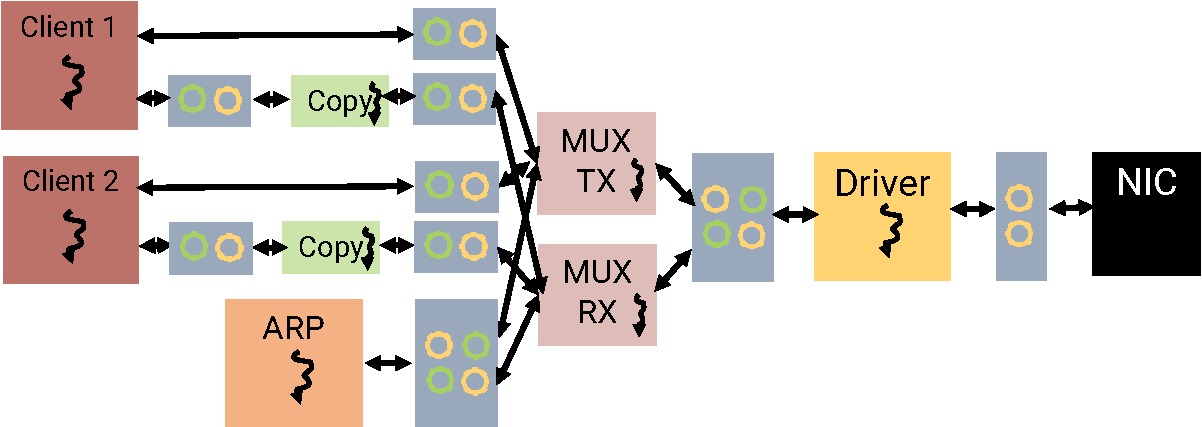
\includegraphics[width=\textwidth]{arp.pdf}
    \caption{Multiple client applications with an ARP component on the sDDF}
    \label{f:arp}
\end{figure}

\subsection{Separate ARP Component}\label{s:arp_design}
A separate ARP component only requires the minimal functionality to respond to 
the Address Resolution Protocol on behalf of any client applications running on
the system. In keeping with the design goals, this component will be kept 
very simple with the aim of enabling formal verification. Consequently, such a goal 
also makes this component easy for developers to reason about and debug. Therefore we consider
this component to be trusted to maintain the integrity of its shared queues with
the multiplexer components as well as interfacing with clients and responding
correctly to ARP on behalf of the clients. \\
While supporting other broadcast protocols, such as DHCP, is out of scope of this thesis, 
the simplicity of the ARP component design enables its functionality to be extended easily
to support other broadcast protocols in the future. Such an extension would entail 
adding additional packet processing logic to our ARP component. 

\section{Client Applications}\label{s:client_apps}

The client application consists of a simple echo server and uses lwIP \cite{Dunkels_01} as an IP
stack library to process the network packet headers. The lwIP API stores packet data, including pointers
to the payload, in a \texttt{pbuf} struct. The \texttt{pbuf}s are allocated from static-sized memory pools and can be chained
together to produce a scatter-gather list.
On the receive path, \texttt{pbuf}s aren't chained together as the incoming payload already contains
all the required packet headers. However, when transmitting a packet via the UDP or TCP API, the \texttt{pbuf} will
only wrap around the actual payload, and in order to add the required headers, lwIP allocates additional \texttt{pbuf}s
containing these headers that are added to the head of a \texttt{pbuf} chain as shown in \autoref{f:pbuf0s}. \\

\begin{figure}[h]
    \centering
    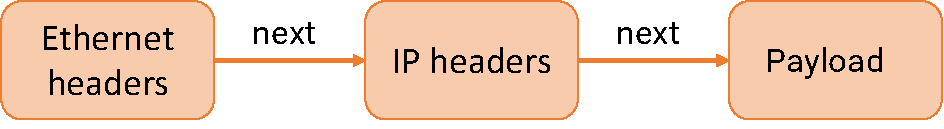
\includegraphics[width=0.6\textwidth]{pbufs0.pdf}
    \caption{Example lwIP \texttt{pbuf} list}
    \label{f:pbuf0s}
\end{figure}

Once a packet is ready to be transmitted,
a chain of \texttt{pbuf}s must then all be copied into a single sDDF buffer before being enqueued to the multiplexer.
The result of this design means that if there isn't a transmit buffer available for this chain of \texttt{pbuf}s, the
packet is dropped and the \texttt{pbuf}s are freed. While this is an acceptable outcome, it unfortunately means that a significant
amount of packet processing is then wasted. In order to combat this on the simple echo server and reduce
wasted cycles, packets are only
processed on the receive path if transmit buffers are available. This stalls the client application
until it receives a notification that more transmit buffers are available. \\

However, this solution is very limiting
as most networking applications do not have symmetric traffic. For example, a client application could receive a
higher number of packets than it transmits, and thus the design stalls the receive processing without reason. 
On the other hand, a client application with higher transmit demands would bypass the check for transmit buffers and result in
packets being dropped after packet processing. \\

To remove the premature check for transmit buffers on the receive path, we need to 
temporarily store the transmit context by storing the \texttt{pbuf} chains when there are not enough transmit buffers
available to the client. Once more transmit free buffers are available (by which the client will be notified),
the client can resume the transmit context. 

\begin{figure}[h]
    \centering
    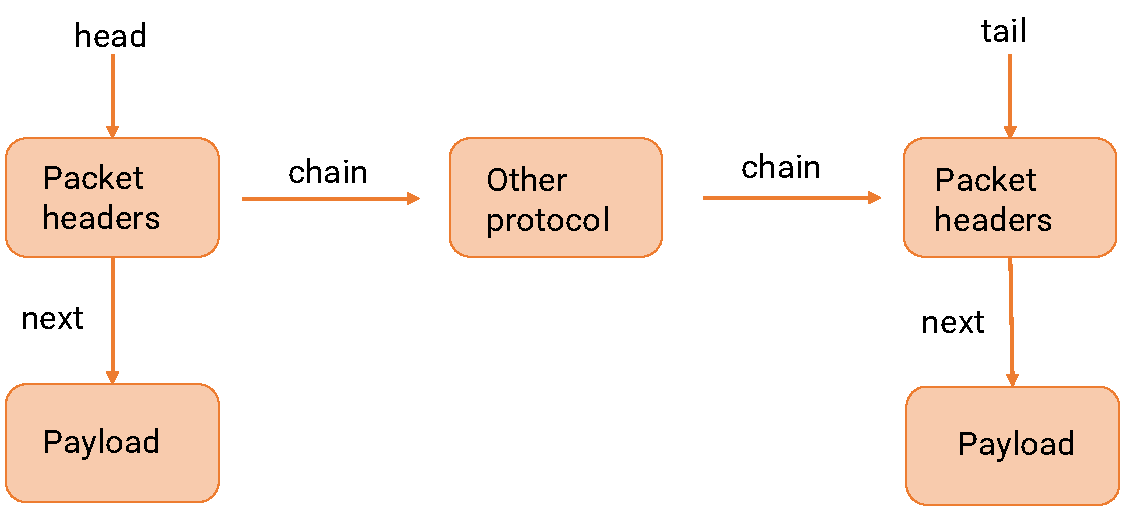
\includegraphics[width=0.7\textwidth]{pbufs.pdf}
    \caption{Example lwIP \texttt{pbuf} chain}
    \label{f:pbufs}
\end{figure}

We store the transmit context by simply linking \texttt{pbuf} chains together and storing the head and tail of the list. 
\autoref{f:pbufs} shows how multiple chains of \texttt{pbuf}s can be linked together. When a chain of pbufs is ready to
be transmitted, but there are not any free transmit buffers, we append the chain to the tail of the list and 
increment the reference count of the chain. This ensures the \texttt{pbuf}s won't be freed until they have actually been sent.
When a client is notified of the availability of more free transmit buffers, we dequeue \texttt{pbuf} chains from the head of
this list. This only requires adding a single extra field to lwIP \texttt{pbuf} structs. This simple change removes any
restriction on the receive path, sets up the client application to no longer expect symmetric traffic. We implement simple, example
applications with asymmetric traffic to evaluate how our framework copes with such loads in \autoref{ch:evaluation}.

\section{Multi-core Systems}\label{s:multicore}

The sDDF is implemented on top of the seL4 microkit, which already supports multicore systems
and so there are minimal changes required
to achieve this. As the transport layer is lock-free and system calls are kept to a minimum, the framework itself 
\emph{should} be capable of exploiting the parallelism of multicore hardware. We explore possible system designs in \autoref{ch:evaluation}.
Furthermore, it is possible to split the driver into two separate components. One component would be responsible for
handling client initiated events (predominantly transmit requests), while the other component would react to 
hardware events. This separation has the potential to achieve more performance on a multicore system as
each of these components could run concurrently on separate cores.\\

\subsection{Two-threaded driver on multi-core systems}
A device driver has multiple tasks: it must react to hardware events as signalled by an interrupt and it must react to software events,
such as a client request. Namely, the driver has 4 tasks:

\begin{enumerate}
    \item Dequeue incoming packets from the hardware receive ring and enqueue them to the RxU queue.
    \item Dequeue free buffers from the RxF queue and enqueue them to the hardware receive ring.
    \item Dequeue used transmit buffers from the TxU queue and enqueue them to the hardware transmit ring.
    \item Dequeue transmitted buffers from the hardware transmit ring and enqueue them to the TxF queue. 
\end{enumerate}

While these tasks involve interfacing with both hardware and software queues, each task involves
producing/consuming to different queues and reacting to different events. Task 3 occurs after a client transmit signal, 
tasks 1 and 4 occur after an interrupt, and task 2 occurs either preemptively after task 1 to ensure the hardware receive
ring is ready to be received, or after a client signal that more free buffers are available. We can split the driver up into
two separate components and simplify the workload as shown in \autoref{f:two_threaded_driver}.

\begin{figure}[h]
    \centering
    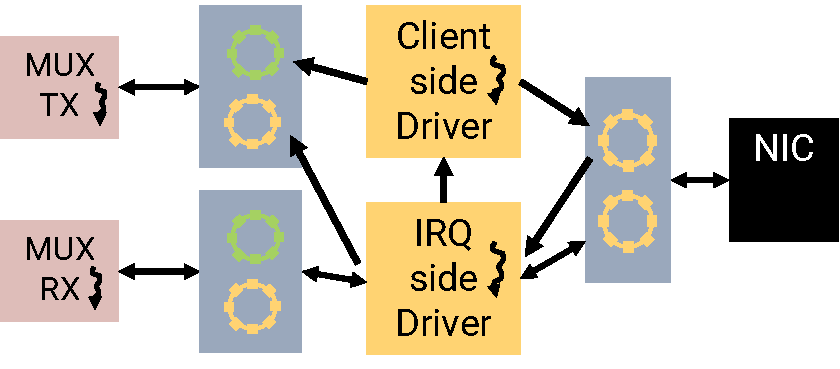
\includegraphics[width=0.6\textwidth]{two_threaded_driver.pdf}
    \caption{Driver architecture with two components}
    \label{f:two_threaded_driver}
\end{figure}

The client side driver is responsible for only task 3. It receives a signal from the transmit multiplexer when packets are ready
to be transmitted, and enqueues them to the tail of the hardware transmit ring. If the hardware transmit ring is full, it waits 
until it receives a notification from the IRQ side driver when space has freed up.\\
However, introducing an additional component to the framework will incur additional performance overheads due to extra context switches required.
We first analyse these overheads in \autoref{ch:evaluation} before concluding whether this design is appropriate on multi-core systems. 

\section{Security}\label{s:security}
Component communication in the sDDF relies on shared memory and asynchronous notifications. While asynchronous communication
has considerable performance benefits (see \autoref{ch:related_work}), it means we trust each component to abide by the protocol. 
Future work, left out of scope of this thesis, will explore verifying all trusted components. However, the system cannot
trust application code. Our design should ensure a 
misbehaving client application does not have the ability to interfere with other clients or the rest of the system.\\

Clients receive data by dequeuing metadata, including buffer addresses, from a shared ring buffer, and transmit data by enqueuing such metadata. 
However, as these shared ring buffers are used by the components on either side of the client (e.g. a multiplexer), we currently 
trust the client to maintain the integrity of the queues, and not write to buffers during DMA (i.e. once a packet has been enqueued
for transmit and before the buffer returns in the free queue). Specifically, we trust the client to:
\begin{enumerate}
    \item Update the tail pointer when dequeuing incoming packets from its RxU queue.\\
    While the rest of this queue can be mapped in as read-only to the client, if the client does not correctly increment this pointer,
    the copy component will incorrectly see this queue as full/empty and potentially could either write over client's data or stop
    enqueuing new packets. As each client application has its own copy component, this potential vulnerability is isolated only to
    the misbehaving client.
    \item Write the correct metadata to the RxF queue once buffers can be recycled.\\ 
    Should a client not do this appropriately, for example, it could give a faulty buffer address/length, the copy component will not 
    use this buffer. This vulnerability is isolated to just the client and its copy component.
    \item Update the head pointer when enqueuing free buffers to its RxF queue.\\
    Like 2., this will only cause the copy component to not reuse newly enqueued buffers.
    \item Signal the copy component after enqueuing free buffers to its RxF queue.\\
    If the client does not inform the copy component of this update and the copy component is blocked on enqueuing incoming packets as there
    aren't enough free buffers to copy into, the copy component may not wake up. This could block any receive traffic to the misbehaving client
    but will not affect other components.\\
    Alternatively, if a client signals its copy component unnecessarily, this has the potential to increase networking latency. 
    As the copy component runs at higher priority than its client, a signal from the client to its copy component will cause an immediate context
    switch. This has the potential to also affect other applications that run at equal or lower priority than the copy component on 
    the same CPU, as they may delayed to be scheduled as a result. seL4 already provides mechanisms to protect against such a scenario in 
    scheduling context objects. We can limit copy components' scheduling parameters such that they will not monopolise the CPU. Then, should 
    a client excessively signal its copier, the copy component will use up its scheduling budget and become blocked, thus reducing any Rx 
    bandwidth to that client. These limits
    will depend on greater system design, in particular, the scheduling parameters of all other applications running on the same CPU.
    \item No longer write data to buffers once enqueued to the clients RxF queue.\\
    Should the client write data to buffers already enqueued in the RxF queue, it will potentially write over incoming data. This will only
    affect the misbehaving client application, but can also be protected against by mapping Rx buffers to clients as read-only.
    \item Enqueue a buffer to the RxF queue only once per use.\\
    If a client enqueues the same buffer multiple times to the RxF queue, it will potentially cause the copy component to write new incoming
    data over other used packets. This may mean the client loses Rx packets. Similarly, this will not affect any other applications.
    \item Write the correct metadata to the TxU queue.\\
    Should the client enqueue faulty metadata, such as a faulty address, the transmit multiplexer can detect this by ensuring the address lies inside
    that clients Tx DMA region, and will refuse this request without impacting any other components.
    \item Update the head pointer of the TxU queue.\\
    If the client does not correctly update this pointer, the multiplexer will not see newly enqueued packets and they may never be sent.
    \item No longer write to the packet after its enqueued to the TxU queue.\\
    Should the multiplexer be responsible for ensuring the packet is well formed with appropriate Ethernet headers, the client could potentially
    alter this data after sanitation and thus potentially send out corrupted packets. While modern NICs are typically equipped to prevent
    such errors, we don't want to always assume the device itself is trustworthy and corrupted packets have the potential to compromise
    other devices on the network.
    \item Signal the transmit multiplexer after enqueuing used transmit buffers.\\
    If the client does not signal the multiplexer, enqueued transmit packets may never be sent. This only affects the client itself.
    Alternatively, if the client signals the Tx multiplexer unnecessarily, it will increase latencies. Similarly to the receive path,
    a signal from client to Tx multiplexer causes an immediate context switch. Unnecessarily invoking the multiplexer will delay other 
    applications running on the same core at lower priority than the multiplexer.
    \item Update the tail pointer of the TxF queue after dequeuing free transmit buffers.\\
    If this is not done and the multiplexer incorrectly sees the queue as non empty, it may write over client data and
    thus potentially overwrite and therefore lose the clients transmit requests. If
    the multiplexer incorrectly sees the queue as full, it will panic. This is because the multiplexer assumes the client's 
    TxF queues are never full (as when it dequeues a new free buffer from the driver, it cannot know in advance where 
    to return the buffer). If one client misbehaves, then it may prevent the multiplexer from dequeuing more free buffers 
    from the driver side and returning them to clients. This has the potential to corrupt the entire transmit path for all
    client applications.
    \item Enqueue a buffer to the TxU queue only once per use.\\
    If a client enqueues the same buffer multiple times to the TxU queue, it will potentially cause the device to send the
    packet multiple times. This may affect lower priority clients by monopolising the device. An appropriate choice of Tx multiplexer
    policy can protect against this consequence, and thus only affecting the misbehaving client.
    \item Keep track of all buffers.\\
    Rx and Tx buffers belong to clients and it is up to the client to not lose buffer pointers. However, should a client lose
    buffers, it could potentially limit that clients available throughput. Clients do not have access to shared buffers so this
    will not affect any other clients.
\end{enumerate}

From the above analysis, and assuming all components other than the client applications are trustworthy,
we can conclude the receive path is secure. A trusted component, the copier, sits between the untrusted client application
and the shared multiplexer, and in each potential vulnerability whereby the client does not abide by the protocol, the copy component
will not enqueue/dequeue more incoming packets and thus starve only the misbehaving client. This assumes the RxU queue between 
the receive multiplexer and copy component is appropriately sized. Should this queue size exceed the number of shared buffers
available for all clients, and a client misbehaves, it could potentially starve other clients. This is because the copier
of a misbehaving client will not enqueue more incoming packets to the client (either temporarily or permanently), and the RxU queue
to the copier could then fill up. If there are limited shared buffers available and a high proportion are enqueued to the copier
of a faulty client, there will be less buffers available for other clients. To prevent such a scenario, we ensure there are enough
shared buffers on the receive path for all RxU queues between the multiplexer and each copy component to be full at the same time.\\

However, the transmit path is not protected from misbehaving client applications. While scenarios 7, 8 and 13 only impact the client
itself, scenario 9 has the potential to compromise other devices on the network without a trusted device, and scenario 11 can block
all transmit traffic, including that of other clients.\\

To remove these vulnerabilities, we can mimic the receive path by injecting a small, trusted component in between each untrusted
client application and the shared multiplexer as shown in \autoref{f:tx_copy}. The component can be configured as
per the system design, or even removed all together, as required by the threat scenario.

\begin{figure}[h]
    \centering
    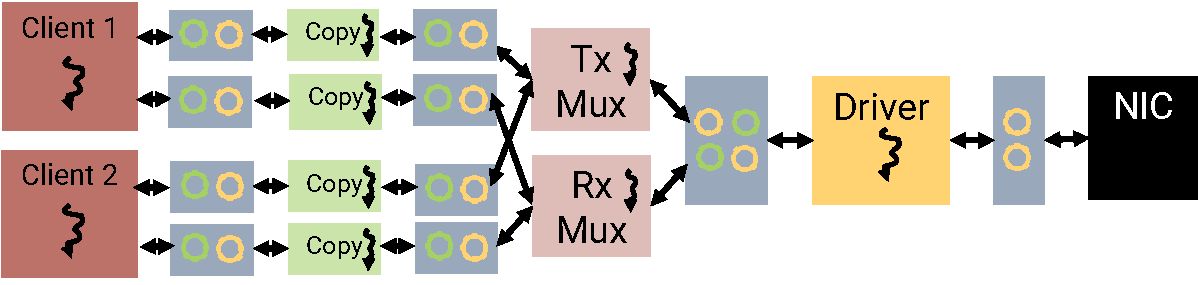
\includegraphics[width=\textwidth]{tx_copy.pdf}
    \caption{Architecture with an additional transmit copy component}
    \label{f:tx_copy}
\end{figure}

To interface with a completely untrusted client application, this new component needs to:
\begin{itemize}
    \item Ensure metadata enqueued to the multiplexer is sane.
    \item If the device is untrusted, check outgoing packets are well-formed and copy them into a separate region not mapped
          into the clients address space.
    \item Interface with the multiplexer correctly by incrementing the head/tail pointers as required.
    \item Ignore any transmit packets that do not abide by the protocols outlined above.
\end{itemize}

Like the receive path copy components, should a client misbehave when interacting with the shared queues, or fail to signal as per
the protocol, the new Tx Copy component will ignore any requests or no longer enqueue free buffers to the client, thus only disturbing
that client and not affecting any other components in the system.\\
Contrary to the Rx Copy component, this does not introduce a shared Tx data region. 
This additional component would introduce some additional performance overheads. These include the cost of reading packet headers, 
an extra system call on the transmit path, and potentially the cost of copying the entire packet. 
We measure these overheads in \autoref{ch:evaluation}.\\
